\documentclass[12pt]{article}
\usepackage{graphicx} % Required for inserting images

\title{Lab 4: Alpha Spectroscopy and Range Measurement}
\author{Owen Strong \\
\itshape Prof.: Angela DiFulvio\\
\itshape TA: Kholod Mahmoud \\
\itshape TA: Shaffer Bauer \\
\itshape TA: Justin Jia \\
}
\date{March 5, 2026 (Adjusted from February 28)}

\usepackage[
    style=ieee
]{biblatex}
\bibliography{refs.bib}

\usepackage[letterpaper, margin=1in]{geometry}
\usepackage{xspace}
\newcommand{\figwidth}{0.75\linewidth}
\newcommand{\halflw}{0.5\linewidth}

% Common Macros
\newcommand{\figref}[1]{Fig.~\ref{#1}}
\newcommand{\defplotW}[3]{
    \begin{figure}[!htb]
        \centering
        \includegraphics[width=#3\linewidth]{fig/#1.png}
        \caption{#2}
        \newcommand{\tmplabel}{fig:#1}
        \label{\tmplabel}
    \end{figure}
}
\newcommand{\defplot}[2]{\defplotW{#1}{#2}{0.75}}
% \newcommand{\defplotJPGW}[3]{
%     \begin{figure}
%         \centering
%         \includegraphics[width=#3\linewidth]{fig/#1.jpg}
%         \caption{#2}
%         \newcommand{\tmplabel}{fig:#1}
%         \label{\tmplabel}
%     \end{figure}
% }
% \newcommand{\defplotJPG}[2]{\defplotJPGW{#1}{#2}{0.75}}

% Specific lab to lab
\newcommand{\micCi}{\xspace$\mathrm{\mu Ci}$\xspace}
\newcommand{\AmSrc}{\xspace$^{241}$Am\xspace}
\newcommand{\PoSrc}{\xspace$^{210}$Po\xspace}


\usepackage{placeins} % FloatBarrier
\usepackage{amsmath} % align
\usepackage{xcolor}
\usepackage[colorlinks=true, citecolor=violet, linkcolor=violet, urlcolor=violet]{hyperref}
\usepackage{enumitem}

\begin{document}
\pagenumbering{gobble}
\maketitle
\pagebreak
{\hypersetup{linkcolor=black}\tableofcontents}
\pagebreak
\pagenumbering{arabic}
\begin{abstract}
A highly important characterizations of radiation interaction with matter is the range of charged particles in matter, and the related property of stopping power.
In this laboratory, we investigated the range and stopping power of 5.468~MeV alpha particles from a 0.1 \micCi \AmSrc source in air, aluminum, and Mylar, as well as geometric attenuation by solid angle, and energy straggling.\\

Using an alpha spectrometer with a vacuum chamber, we measured 3-minute transmission spectra of alpha particles through five thicknesses each of air, aluminum, and Mylar, and used the peaks of these spectra to characterize ranges and stopping power.
We compared these data to ranges, stopping powers, and transmission spectra generated using the codes SRIM and TRIM.\\

We estimated ranges of $21\pm4$~mm in air, $36\pm9$~microns in aluminum, and $9.0\pm1.8$~microns in Mylar.
We observed ranges in air and Mylar drastically lower than SRIM ranges, while the range in aluminum was more comparable.
Likewise, we found stopping powers using TRIM data of air and Mylar in excess of SRIM stopping powers, while aluminum stopping powers were incalculable using experimental or TRIM data due to low transmission through assessed thicknesses of the material.
In the same SRIM data, we observed a strong dominance of electronic stopping power in the total stopping power of alpha particles for all three materials.\\

We were unable to characterize the geometric attenuation of the measurements in air, with theoretical solid angle calculations still yielding normalized intensities through vacuum which decreased over the same distances from the detector.
We observed noticeable energy straggling in the TRIM-generated spectra of transmitted alpha particles through the materials, having wider distributions of energy the more drastically attenuated particles were.\\

These results demonstrate the importance of experimental setup parameters such as material thickness choice and handling, solid angle normalization, vacuum production, and comparison with theoretical data in assessing range and stopping power, and may be of use to those either working with similar ions and materials, or wishing to investigate ion stopping power and ranges in materials.
\end{abstract}

\section{Introduction and Background}
\interfootnotelinepenalty=10000
A key metric of interest for radiation in matter is range, that is, the depth along the initial direction which a particle is expected, on average, to penetrate through a material.
For a given type of particle, this range is further highly dependent on an incident particle's energy and the electron/neutron densities of the medium.\cite{npre_lab_4_manual_2025}
This range is related to another property of interest: stopping power, or the loss of energy as a charged particle travels through a medium.\\

This laboratory investigates the range and stopping power of alpha particles, as emitted by \AmSrc, through aluminum metal, Mylar\footnote{While material names are usually kept in lowercase, ``Mylar'' is a brand name, and remains accordingly capitalized in this report.} plastic, and air, in experimental data compared to computer-generated data.
More broadly, the energy loss phenomena of alpha particles through different materials, including energy straggling, and the effects of geometric attenuation corresponding to solid angle, are also investigated.
\subsection{Charged Particle Energy Loss}

As charged particles travel through a material, they lose energy.
This loss can be quantified by the stopping power of the material.
This stopping power can be understood as the energy lost per unit distance traveled, and is denoted $-dE/dx$.
The two primary mechanisms by which this loss occurs are Coulomb interactions with electrons in the material, causing constant small deflections and loss, and Coulomb collisions with nuclei, which are rarer but can cause much greater deflection and loss.
This relationship is thus denoted:
\begin{equation}\label{eq:stop-split}
    \left(-\frac{dE}{dx}\right)_{total}=\left(-\frac{dE}{dx}\right)_{electronic} + \left(-\frac{dE}{dx}\right)_{nuclear}
\end{equation}
This negative sign is often included by convention, to consider stopping power as a positive quantity, where $dE/dx$ itself is necessarily negative as the energy decreases through material.
An example comparison of electronic and nuclear stopping powers across different energies of alpha particles in iron may be seen in \figref{fig:intr0-ironstop}.\\

\defplot{intr0-ironstop}{The electronic and nuclear stopping powers for alpha particles in iron. Figure sourced from lab manual.\cite{npre_lab_4_manual_2025}}

The projected range $R_p$ of a particle with energy $E$ can then be found by integrating total stopping power from starting energy to complete loss of energy $E\rightarrow0$:
\begin{equation}\label{eq:range}
    E_p = \int_0^{R_p}dx = \int_E^0\frac{dE'}{\frac{dE}{dx}(E')}
\end{equation}
With correct stopping powers, Equation~\ref{eq:range} could be used to calculate the range of a particle, or a numerical simulation such as  Monte Carlo code could be used to determine the range to compare with experimental data.\\

In this laboratory, the SRIM (Stopping and Range of Ions in Matter) and TRIM (Transport and Range of Ions in Matter, included within SRIM) codes are used to generate these estimations.
TRIM is a Monte Carlo code which simulates the energy loss of individual ions through a wide variety of materials and compounds, which can be compared to experimental observations.
\FloatBarrier
\section{Experimental Procedure}\label{sec:methods}
In this section, we detail the equipment used and experiments performed in this laboratory. 
\subsection{Equipment}
In this laboratory, we employed an alpha spectrometer attached to a vacuum pump, with a silicon surface barrier detector biased by a high voltage power supply (HVPS), a multichannel analyzer (MCA), a 0.1 \micCi alpha particle source, five 18 micron thick sheets of aluminum, five 3.6 micron thick sheets of Mylar, and a computer with the softwares Maestro and SRIM/TRIM installed.
Further equipment details, where applicable, may be found in Appendix~\ref{app:equip}.

\subsection{Setup}
\FloatBarrier
We constructed a system according to \figref{fig:Lab4_diag} to observe alpha particle energy spectra from a source in a controlled environment, which can be seen in \figref{fig:Lab4_setup}.

\defplot{Lab4_setup}{The experimental setup used during the laboratory.}
\defplot{Lab4_diag}{A system diagram of the laboratory setup.}

\FloatBarrier
\subsection{Experiments 1 and 2: Measuring Alpha Particle Range and Stopping Power in Vacuum and Air}
\FloatBarrier
We first biased the detector to $+60$~V.
As the detector is a silicon surface barrier detector, we took care to apply the bias slowly and in small steps, to avoid potential plasma ionization which would damage the detector.\\

% \defplotJPGW{Lab4_chamber}{The chamber of the alpha spectrometer module, with the source mounted on a plate in one of several available vertical slots, and the cylindrical detector overhead.}{0.4}
\begin{figure}
    \centering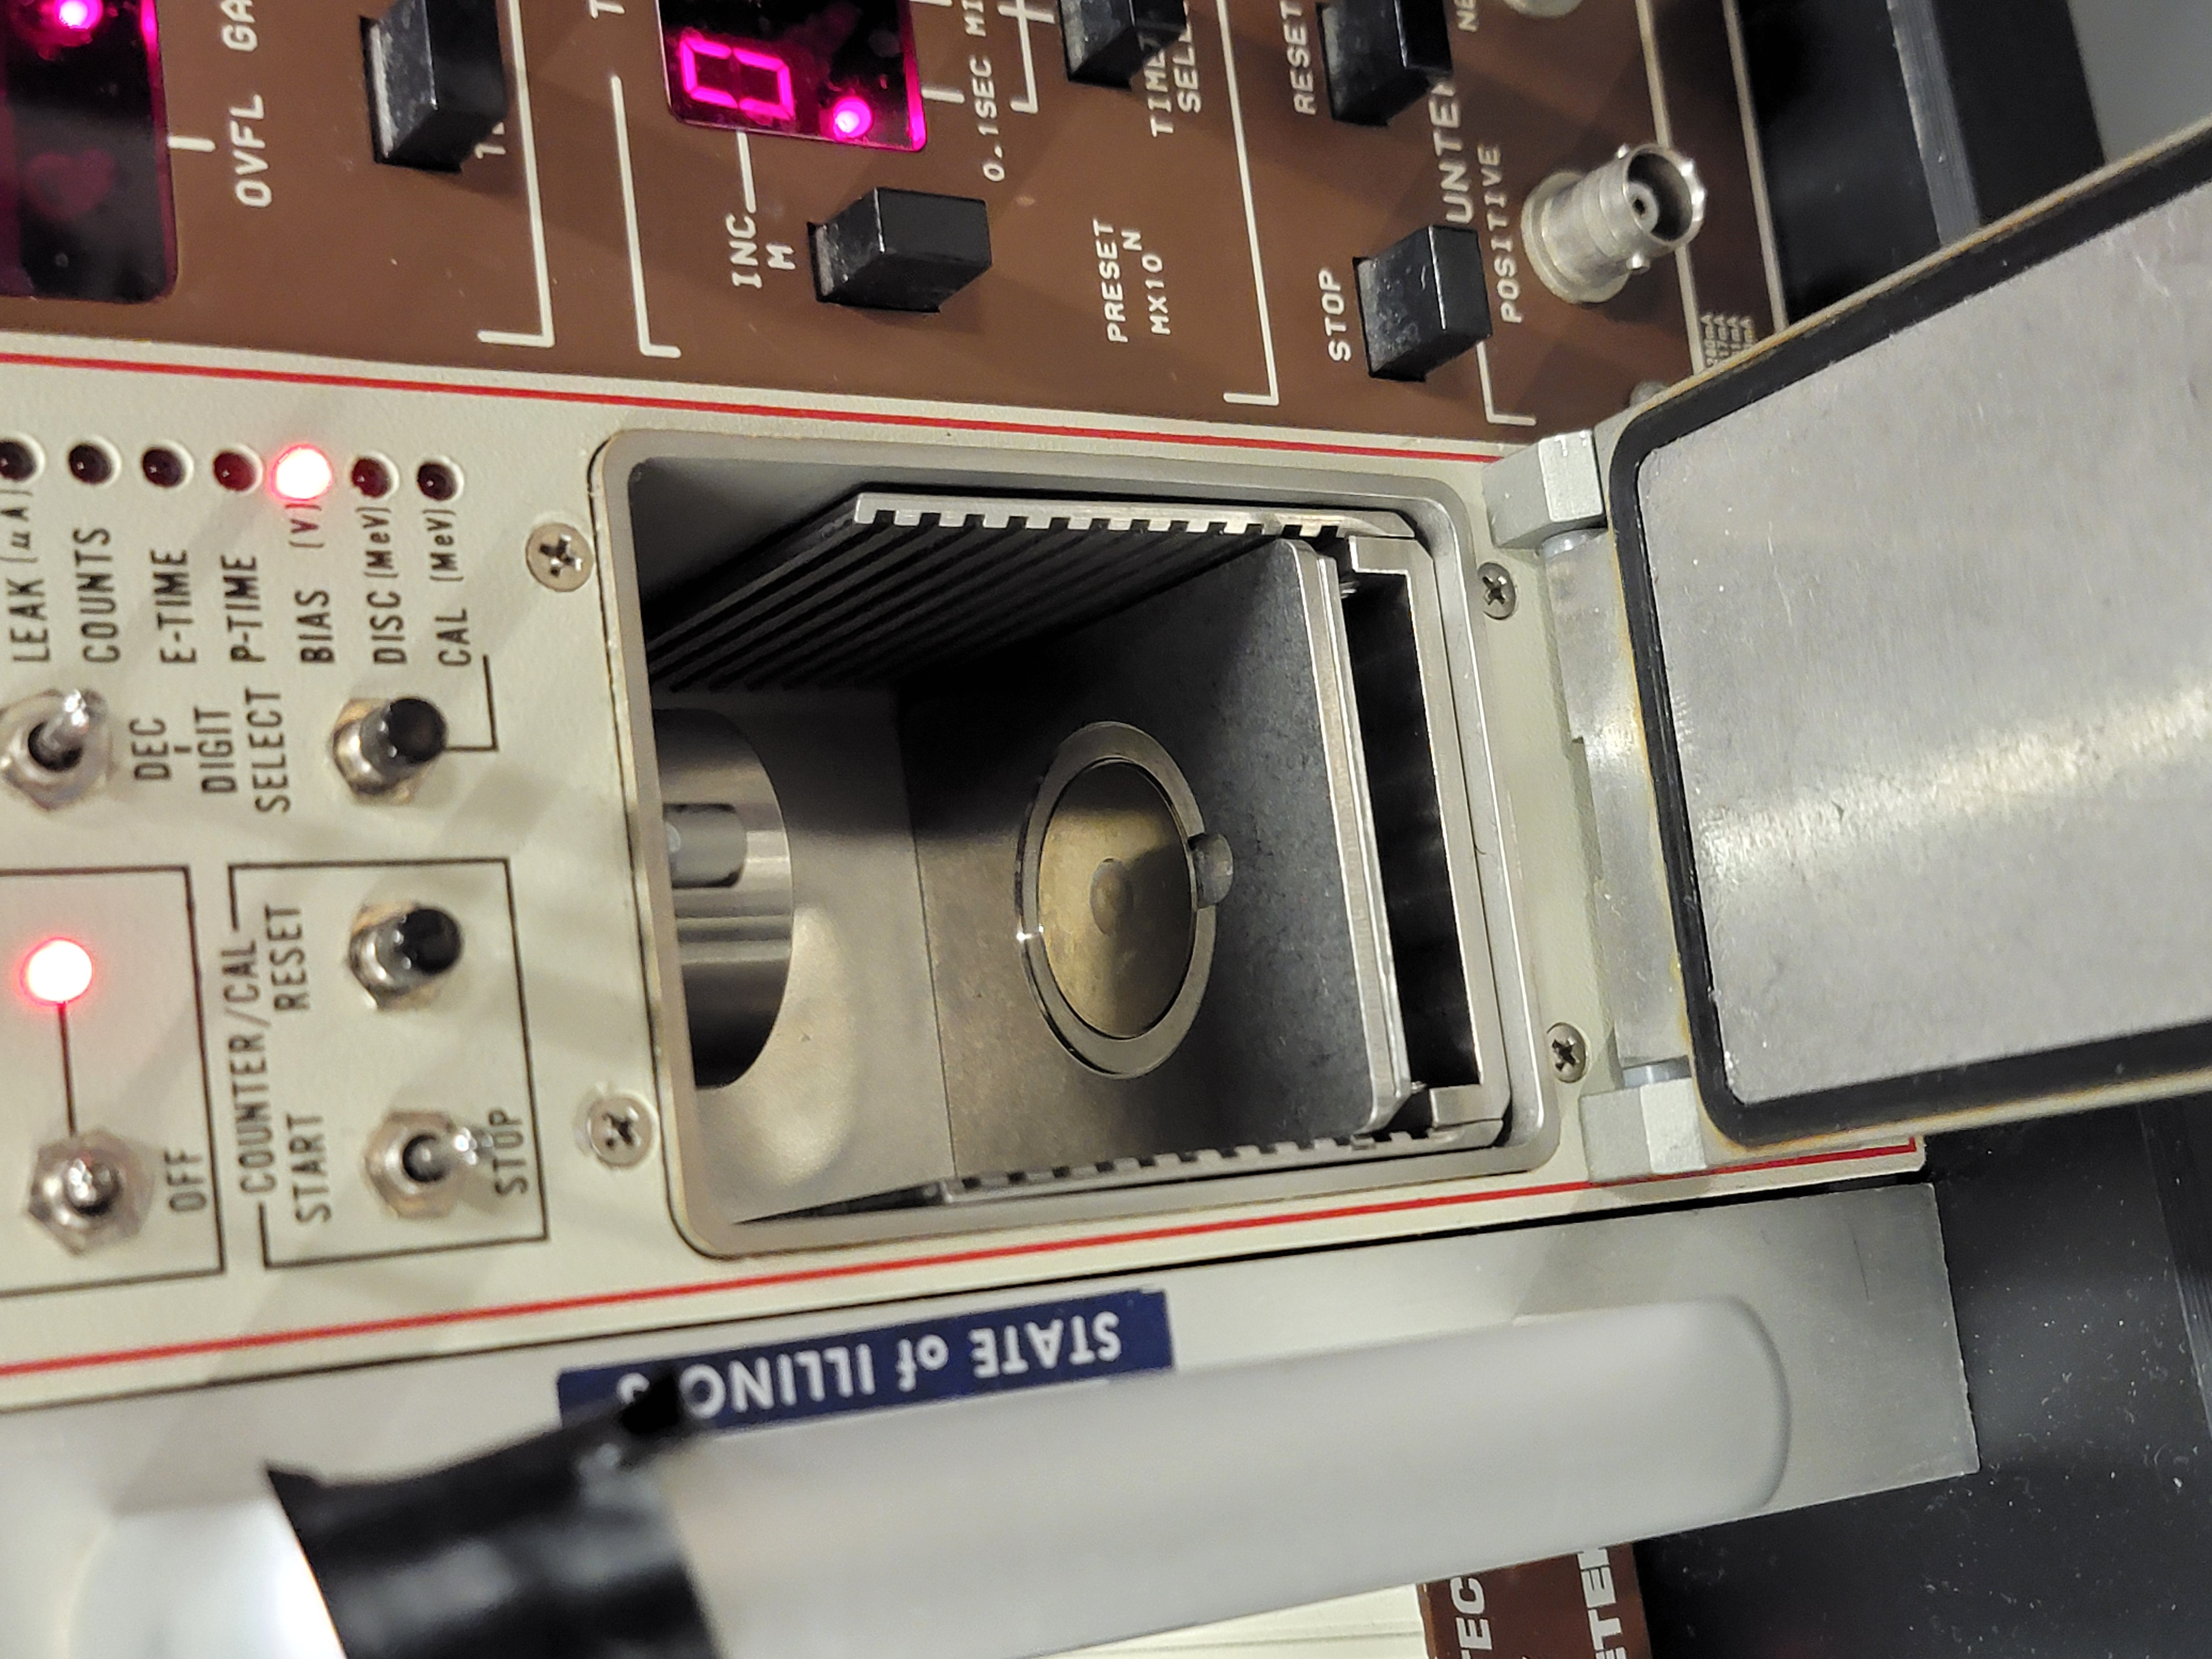
\includegraphics[width=0.4\linewidth,angle=-90]{fig/Lab4_chamber.jpg}
    \caption{The chamber of the alpha spectrometer module, with the source mounted on a plate in one of several available vertical slots, and the cylindrical detector overhead.}
    \label{fig:Lab4_chamber}
\end{figure}

Mounting the source in the lowest possible slot in the chamber, as seen in \figref{fig:Lab4_chamber}, we closed the chamber door and evacuated the chamber using the attached vacuum pump.
We then, using Maestro on the computer, started recording the energy spectrum observed by the detector, and recorded for a period of 3 minutes.
Then, releasing the vacuum in the chamber, we analogously recorded the spectrum over 3 minutes in air.
We additionally recorded the distance of the source from the detector, using the known locations of the 12 vertical slots in the chamber relative to the location of the detector.\\

We repeated this spectrum measurement in vacuum and in air four more times at different slots, conducting a total of ten spectrum measurements at distances of 49, 33, 25, 17, and 1 mm from the detector.\\
\FloatBarrier
\subsection{Experiments 3 and 4: Measuring Alpha Particle Range and Stopping Power in Mylar and Aluminum}
\FloatBarrier
We selected a slot location corresponding to a distance approximately 4 cm from the detector, and placed the source plate in this slot.
We covered the source with a single 3.6 micron thick sheet of Mylar, using a washer to hold it steady over the source as shown in \figref{fig:Lab4_mylar}.\\

With the source under Mylar in the chamber, we evacuated the chamber and performed a 3-minute spectrum measurement for the single Mylar sheet, and then repeated this process with two, three, four, and five sheets of Mylar, ensuring the source remained at a constant distance from the detector through the series of spectrum measurements, to build a series of spectra with attenuation through five distances in Mylar.\\

We then repeated this process for up to five sheets of aluminum foil.
A setup with aluminum foil over the source with a washer to hold steady may be seen in \figref{fig:Lab4_al}.\\

\begin{figure}
    \centering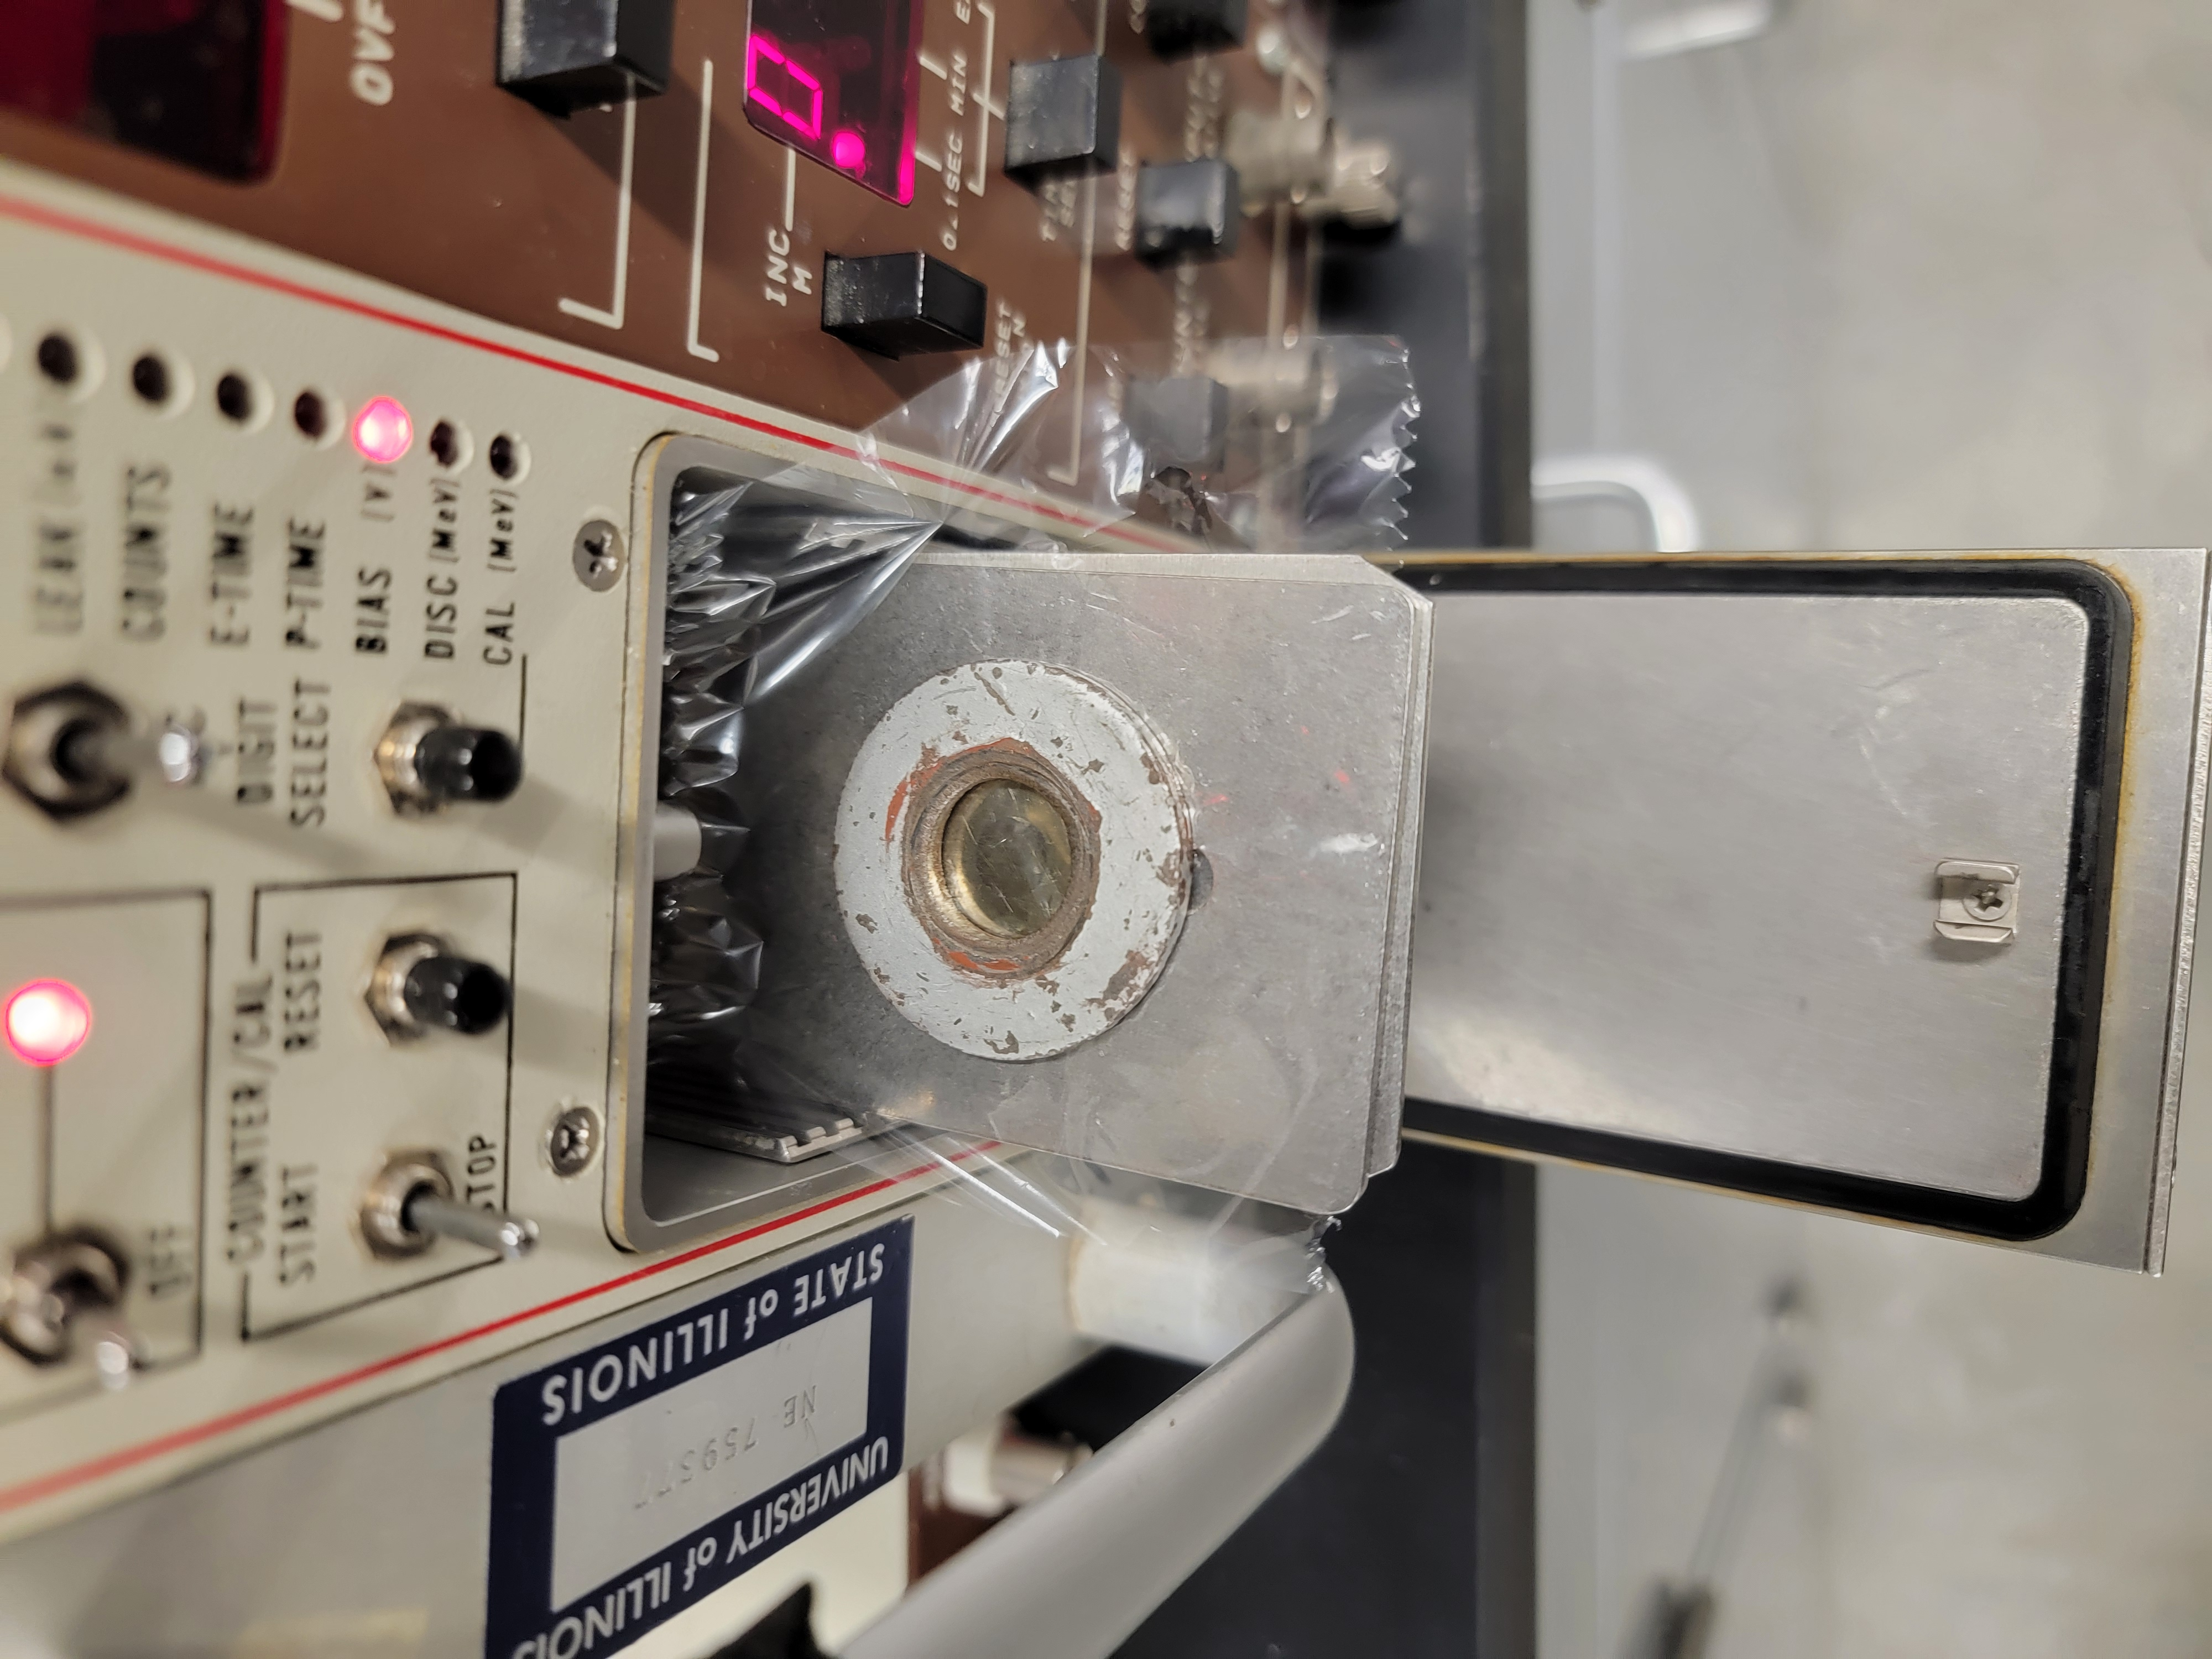
\includegraphics[width=0.4\linewidth,angle=-90]{fig/Lab4_mylar.jpg}
    \caption{The alpha source covered by one sheet of 3.6 micron thick Mylar, with a washer to hold it in place.}
    \label{fig:Lab4_mylar}
\end{figure}

% \defplotJPGW{Lab4_al}{The alpha source covered by one sheet of 18 micron thick aluminum foil, with a washer to hold it in place.}{0.4}
\begin{figure}
    \centering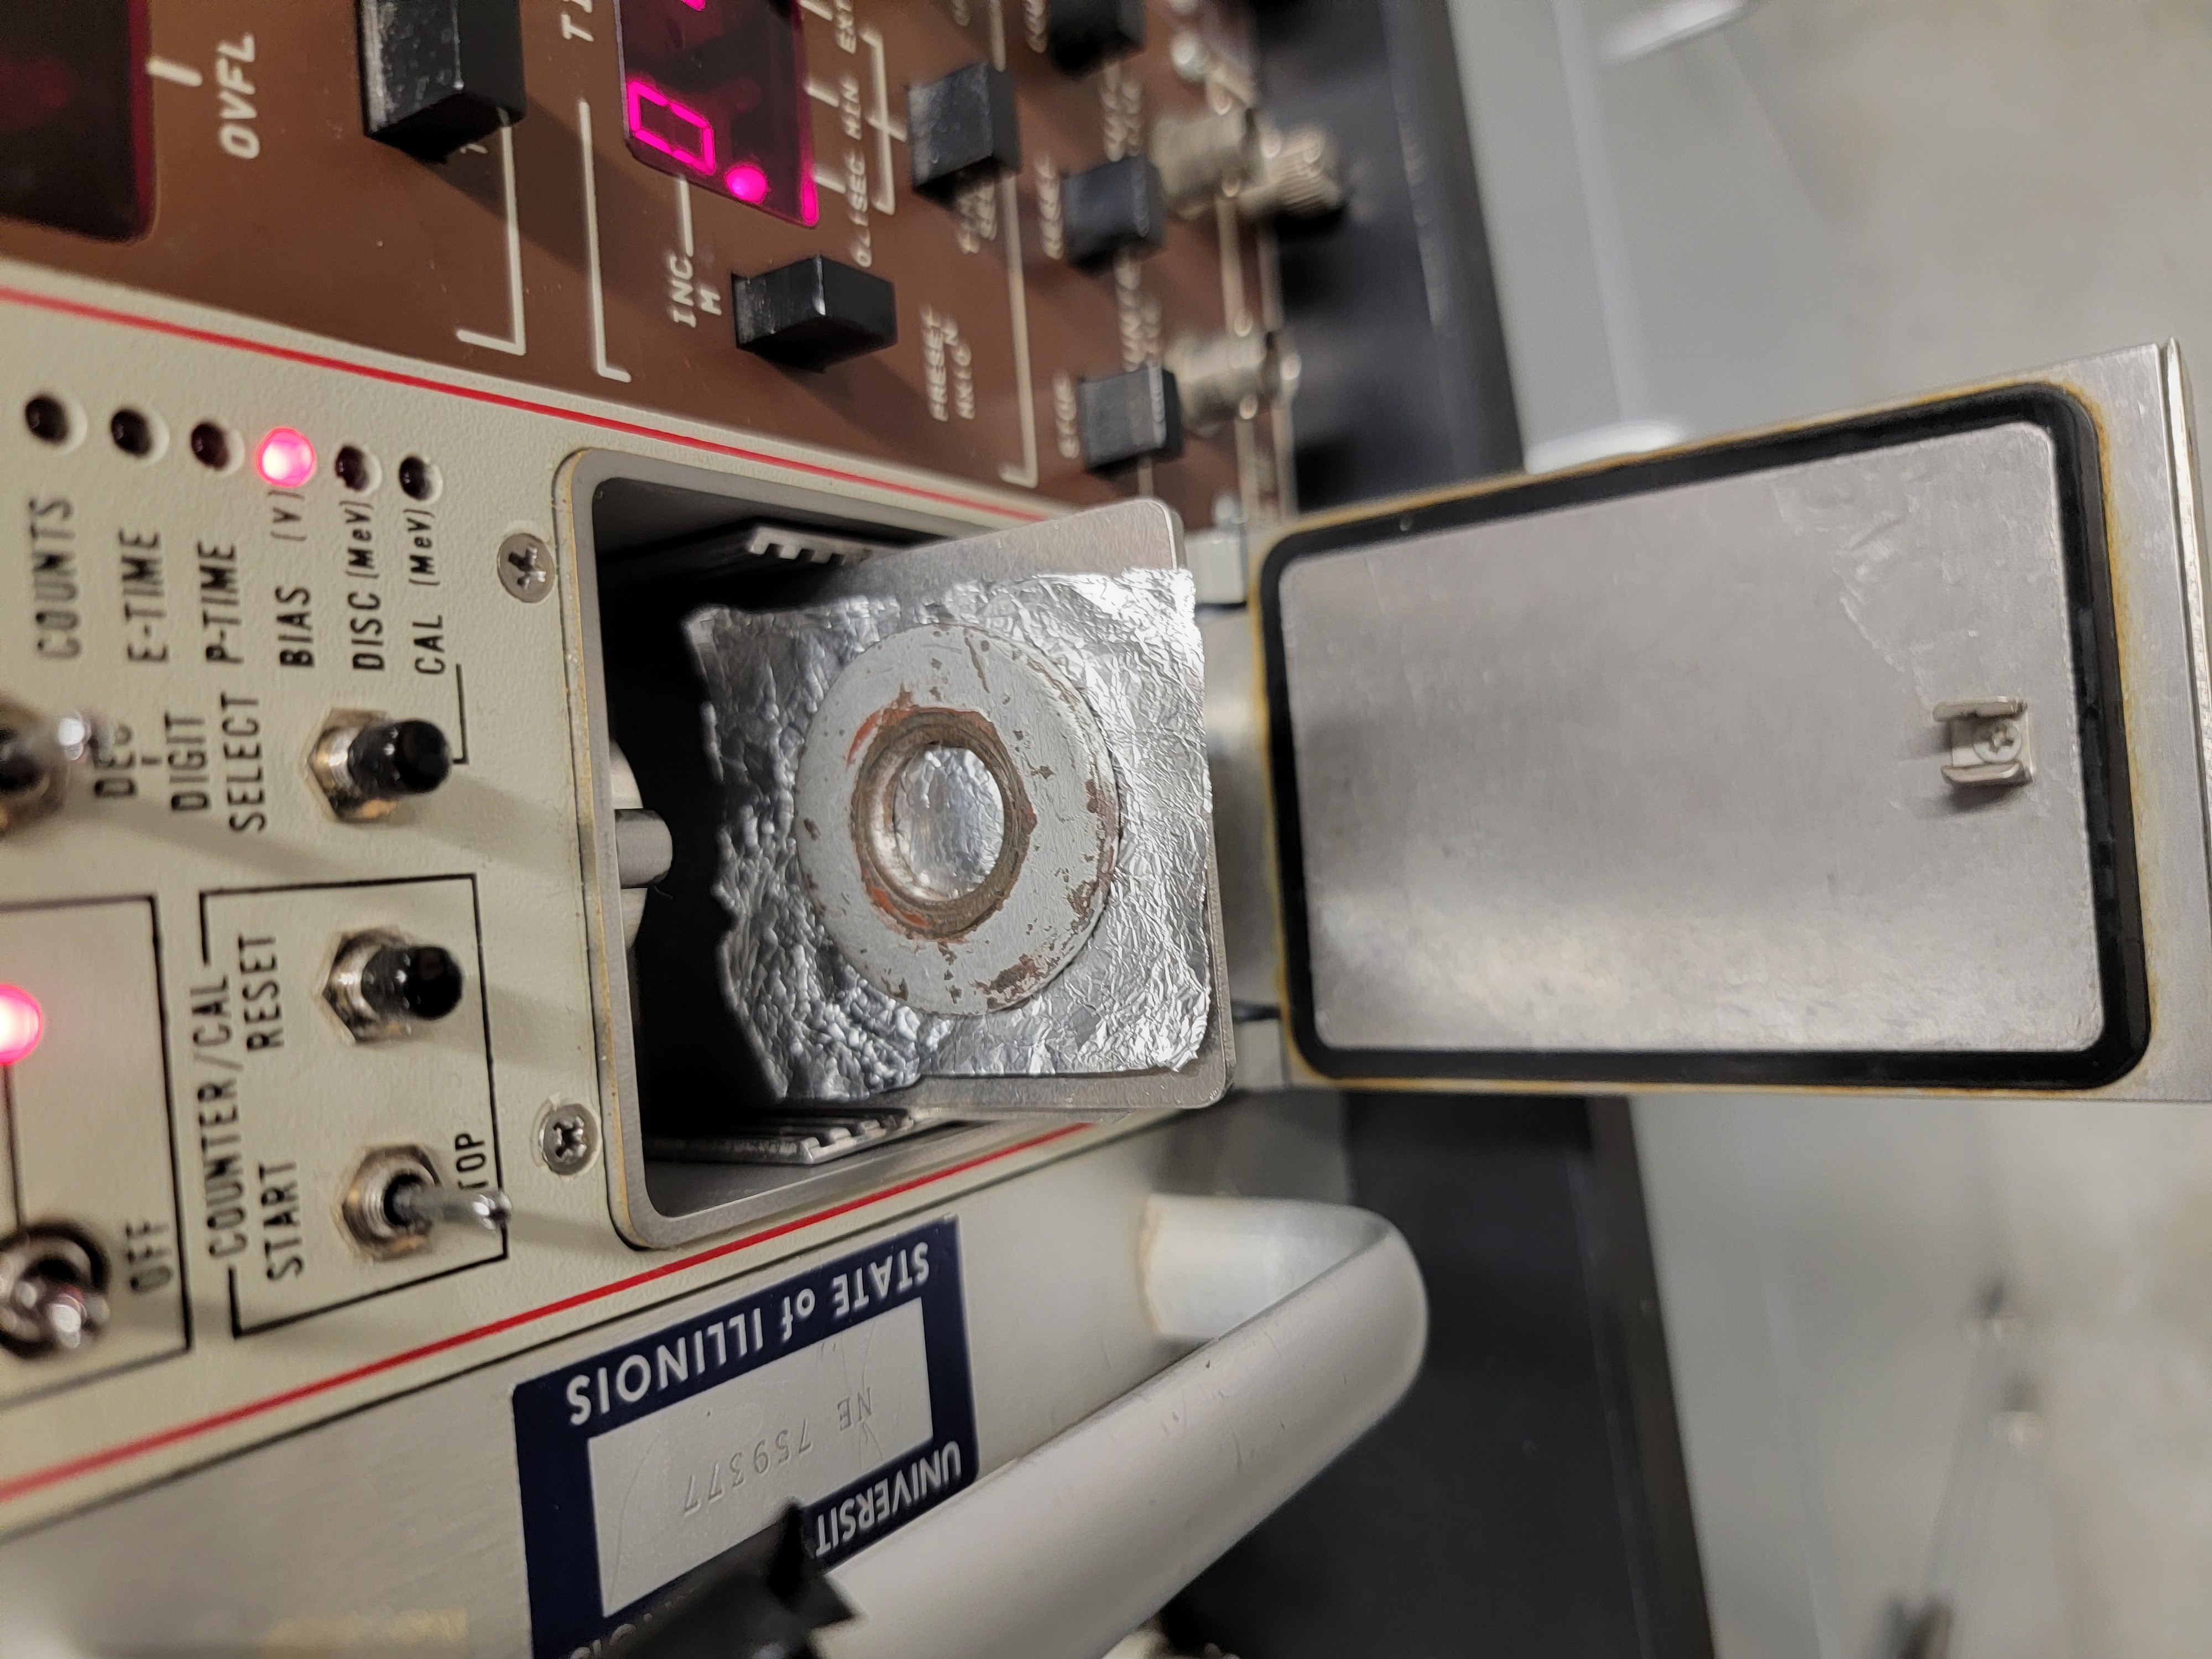
\includegraphics[width=0.4\linewidth,angle=-90]{fig/Lab4_al.jpg}
    \caption{The alpha source covered by one sheet of 18 micron thick aluminum foil, with a washer to hold it in place.}
    \label{fig:Lab4_al}
\end{figure}

After conducting all measurements, we released the vacuum in the chamber, removed the source, and slowly unbiased the detector.

\FloatBarrier
\subsection{Estimating Ranges with SRIM}
We then used the software SRIM to calculate tables of stopping power and range for different energies of alpha particles in air, Mylar, and aluminum.\\

To calculate stopping power and range for a material, we opened SRIM and selected Stopping/Range Tables.
We selected helium ions (i.e., alpha particles) with energy ranging from 10~keV to 10~MeV (encompassing the \AmSrc particle energy of 5.486~MeV), and selected the material, either as an element (for aluminum), or using the compound dictionary (for Mylar and for air).\\

Selecting units of stopping power in eV per Angstrom (lower left box), we then clicked the Calculate Table button and saved the output, containing stopping powers and ranges for different energies in each material.

\subsection{Calculating Energy Distribution of Transmitted Ions through Materials in TRIM}

We then used the software TRIM to calculate the energy distribution of ions transmitted through different thicknesses of each material.\\

Opening the main SRIM menu, we selected TRIM calculation.

We specfified an ion type of He for alpha particles, an energy of 5.486~Mev corresponding to the \AmSrc source, and entered the specific material's composition as with the SRIM calculations above.\\

In the output disk files box near the bottom middle of the menu, we selected the ``Transmitted ion'' option to write a table of all transmitted ions to a file, and we specified to write into a new TRANSMIT file.\\

We then specified the target width to the desired thickness of the material to simulate, specified for TRIM to simulate 1000 ions in the lower left portion of the window, and started the TRIM run by pressing Save Input and Run TRIM.\\

We then named and copied the TRANSMIT file produced to a different location, before repeating for the next combination of material and thickness.
In this way, we used TRIM to simulate alpha particle transmission through each of the experimentally tested thicknesses of air, aluminum, and Mylar.
\subsection{Range Estimation from Transmission Data}


\FloatBarrier
Since particles may not stop at exactly the same distance, to practically estimate the range of the particle and energy, we estimate the range of a particle as the distance where only half the particles are transmitted, as seen in \figref{fig:mat0-range}.\\

\defplotW{mat0-range}{An estimate of range as the distance where $N/2$ of the original $N$ particles have been attenuated by the medium. Figure sourced from \emph{Measurement and Detection of Radiation}.\cite{tsoulfanidis_measurement_2015}}{0.5}

In lieu of exact particle transmission rates, we then estimate this by the distance where peak intensity drops to half that of that measured for the lowest distance.
\FloatBarrier
\section{Experimental Results}\label{sec:results}\FloatBarrier

In \figref{fig:vac_dist_v_I}, the integrated count rate for the alpha source is shown after attenuation through different distances in vacuum. 
However, to does not account for the geometric attenuation, one must first normalize by solid angle $\Omega$, using the following formula\cite{knoll_radiation_2010}:
\begin{equation}\label{eq:sangle}
    \Omega=2\pi\left(1-\frac{d}{\sqrt{d^2+a^2}}\right)
\end{equation}
where $d$ is the distance of the (point) source from the detector, and $a$ the diameter of the detector, a sufficiently long cylinder.
This formula assumes the point source is centered on the cylindrical detector's axis.\\

If the source can ``see'' $\frac{\Omega}{4\pi}$ of the detector, then dividing by this fraction yields an intensity normalized by solid angle.
\figref{fig:vac_dist_v_nI} shows the integrated count rate for distances through vacuum, normalized by solid angle, compared to the original rates.\\


\defplot{vac_dist_v_I}{The integrated peak intensity of the alpha source after attenuation through varying distances in vacuum.}
\defplot{vac_dist_v_nI}{The integrated peak intensity of the alpha source after attenuation through varying distances in vacuum, both raw and after normalizing by visible solid angle.}

In Figs.\ref{fig:air_dist_v_nI} through \ref{fig:air_dist_v_FWHM}, attenuation over distance in air can be observed through effects on integrated peak intensity (both gross and normalized rates), energy, and full width half maximum (FWHM) of energy peaks.
Normalized peak intensity appears to reach half that of the first measurement between the measurements at 17 and 25 mm, yielding a range estimate of $21\pm4$~mm for 5.486 MeV alpha particles in air. 
\\

\defplot{air_dist_v_nI}{The integrated peak intensity of the alpha source after attenuation through varying distances in air, both raw and after normalizing by visible solid angle.}
\defplot{air_dist_v_E}{The peak energy after attenuation through different distances in air.}
\defplot{air_dist_v_FWHM}{The full width half maximum of peak energy after attenuation through different distances in air.}

The attenuation through aluminum, also shown through effects on peak intensity, peak energy, and peak FWHM, are shown in Figs.~\ref{fig:Al_thick_v_I}, \ref{fig:Al_thick_v_E}, and~\ref{fig:Al_thick_v_FWHM}.
Figs.~\ref{fig:My_thick_v_I}, \ref{fig:My_thick_v_E}, and~\ref{fig:My_thick_v_FWHM} show the same for Mylar.
Intensity appears to halve around 36 microns of aluminum, and with measurements every 18 microns, this yields a range estimate of $36\pm9$~microns in aluminum.
For Mylar, peak intensity drops below half between 7.2 and 10.8 microns, yielding a range estimate of $9.0\pm1.8$~microns.
\\

\defplot{Al_thick_v_I}{The integrated peak intensity after attenuation through varying thicknesses of aluminum.}
\defplot{Al_thick_v_E}{The peak energy after attenuation through varying thicknesses of aluminum.}
\defplot{Al_thick_v_FWHM}{The full width half maximum of peak energy after attenuation through varying thicknesses of aluminum.}

\defplot{My_thick_v_I}{The integrated peak intensity after attenuation through varying thicknesses of Mylar.}
\defplot{My_thick_v_E}{The peak energy after attenuation through varying thicknesses of Mylar.}
\defplot{My_thick_v_FWHM}{The full width half maximum of peak energy after attenuation through varying thicknesses of Mylar.}

For three layers of Mylar, and to a lesser extent for four and five, a bifurcation of the dominant peak was also observed, as shown in \figref{fig:My3_bifur}.
\defplot{My3_bifur}{Bifurcation of the dominant spectrum peak for three layers of Mylar.}

\FloatBarrier
Using the simulated data of 5.486~MeV alpha ion transmission in dry air, aluminum, and Mylar in TRIM, rough estimates of total stopping power $-dE/dx$, using an estimate of the derivative between adjacent measurements of energy $E$ and $x$:
\begin{equation}\label{eq:dedx}
    -\frac{-dE_{i+\frac{1}{2}}}{dx_{i+\frac{1}{2}}}\approx\frac{E_i-E_{i+1}}{x_{i+1}-x_i}
\end{equation}
where $E_{i+\frac{1}{2}}=\frac{1}{2}(E_i+E_{i+1})$.
Using equation~\ref{eq:dedx}, estimates of total stopping power $-dE/dx$ can be observed in \figref{fig:air_dEdx} and \figref{fig:My_dEdx}.
For aluminum, TRIM did not calculate any ions being successfully transmitted through more than 1 layer, and so no stopping power estimate could be made this way.\\

\defplot{air_dEdx}{The total stopping power of 5.486MeV alpha particles in air, estimated using energy attenuation at five distances calculated by TRIM.}
\defplot{My_dEdx}{The total stopping power of 5.486MeV alpha particles in Mylar, estimated using energy attenuation at five distances calculated by TRIM.}

\FloatBarrier

Using SRIM, we calculated nuclear, electron, and total stopping powers for alpha particles ranging in energy from 10~keV to 10~MeV.
These are plotted in \figref{fig:air_SRIM} for air, \figref{fig:Al_SRIM} for aluminum, and \figref{fig:My_SRIM} for Mylar.\\

\defplot{air_SRIM}{The nuclear, electron, and total stopping powers of air for alpha particle ions of energies ranging from 10~keV to 10~MeV, calculated using SRIM, compared to the total stopping power estimated from transmission data.}
\defplot{Al_SRIM}{The nuclear, electron, and total stopping powers of aluminum for alpha particle ions of energies ranging from 10~keV to 10~MeV, calculated using SRIM.}
\defplot{My_SRIM}{The nuclear, electron, and total stopping powers of Mylar for alpha particle ions of energies ranging from 10~keV to 10~MeV, calculated using SRIM, compared to the total stopping power estimated from transmission data.}

\FloatBarrier

Likewise, we calculated the projected range of alpha particles with energies ranging from 10~keV to 10~MeV using SRIM.
\figref{fig:air_range} compares these ranges to the range for 5.486~MeV alpha particles in air, while \figref{fig:AlMy_range} compares these for aluminum and Mylar.

\defplot{air_range}{The range of alpha particles between 10~keV and 10~MeV in energy in air, calculated using SRIM, compared to the 5.486~MeV range estimated using experimental attenuation.}
\defplot{AlMy_range}{The range of alpha particles between 10~keV and 10~MeV in energy in aluminum and Mylar, as calculated using SRIM, compared to the 5.486~MeV ranges estimated using experimental attenuation.}

\FloatBarrier

The energy spectra of 5.486 MeV alpha particles transmitted through various distances in air, aluminum, and Mylar can be compared in \figref{fig:combined-spectra}.

\begin{figure}
    \centering
    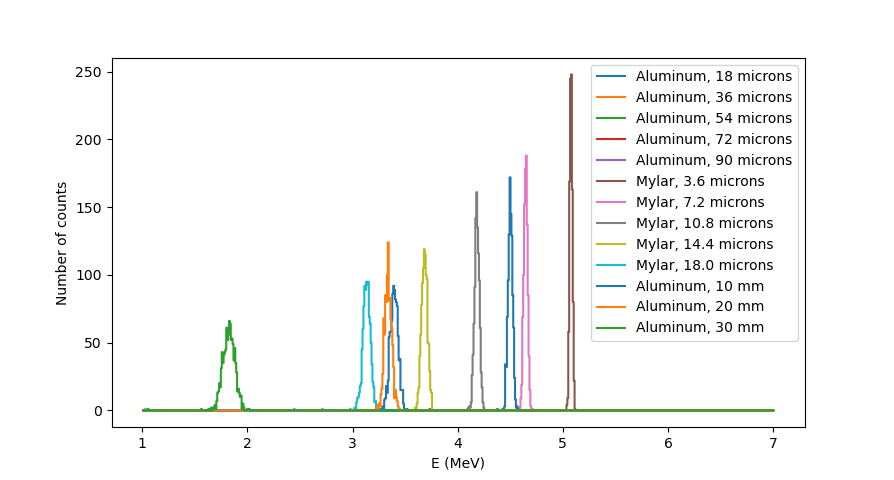
\includegraphics[width=\linewidth]{fig/combined_spectra.png}
    \caption{Energy spectra of 5.486 MeV alpha particles transmitted through various thicknesses of air, aluminum, and Mylar.}
    \label{fig:combined-spectra}
\end{figure}

\FloatBarrier\section{Discussion}\label{sec:disc}
The solid angle calculation of Equation~\ref{eq:sangle} are expected to normalize the intensity measured between measurements with the source different distances away from the detector.
However, this is not what is observed.
In \figref{fig:vac_dist_v_nI}, while normalization makes the ratios between the different distances' integrated intensity less drastic, it does not remove the relationship of these intensities to the distances they were taken at in vacuum, with further distances still resulting in substantially lower peak intensity.
This might result from a lack of a perfect vacuum being drawn, but might also reflect an imperfect accounting for solid angle.
For example, while Equation~\ref{eq:sangle} treats the source as a point source perfectly aligned with the cylindrical detector's axis, it is possible the source is large enough or was far enough off-axis to affect this approximation.\\

The ranges estimated for 5.486~MeV alpha particles using experimental data varied in accuracy.
In \figref{fig:air_range}, we estimate a range in air substantially lower than that calculated by SRIM.
If our solid angle normalization were imperfect in a way that further decreased intensity by distance than we expected, this might result in such an underestimate in range.
The range in Mylar (\figref{fig:AlMy_range}) was also drastically underestimated, but since these measurements were taken at the same distance, solid angle calculations would not account for this error.
Instead, it is still possible that source location shifted more than trivially between measurements, or that wrinkles in the somewhat unwieldy Mylar sheets resulted in greater thickness than expected.
Another explanation may be in difficulty reading the spectra of Mylar: it is possible that the bifurcation of the peak for three layers lead to a drastic underestimate of integrated intensity for this thickness of Mylar, leading to a substantial underestimate in range.

In the same figure, we observe a seemingly more accurate estimation of range in aluminum, but a much more substantial error.
This error reflects a large difference in thickness between different measurements, and suggests we did not have thin enough sheets of aluminum to precisely estimate the range of 5.486~MeV alpha particles in aluminum.\\

While total stopping power could not be estimated with transmission data for aluminum, the estimates for Mylar and air both seemed to consistently overestimate compared to SRIM data.
While this is consistent with our experimental ranges in both materials being lower than SRIM data, it is unlikely that experimental flaws, like altered detector position, solid angle calculations, or Mylar distortions would affect these stopping power estimates, given that we conducted these estimates using TRIM data over the experimental data.
It is possible that our estimate of $-dE/dx$ using Equation~\ref{eq:dedx} is flawed, especially for such drastic differences in thickness and energy attenuation.\\

We observe substantial energy straggling in the transmitted alpha particle energy spectra generated by TRIM, seen in \figref{fig:combined-spectra}.
As expected, rather than consistently decaying to one precise energy, we see a distribution of energies around a central peak, and this peak widens the more the ions are attenuated (i.e., to lower energy $E$).\\

From the SRIM stopping power calculations in Figs.\ref{fig:air_SRIM}, \ref{fig:Al_SRIM}, and~\ref{fig:My_SRIM}, we see that 5.486~MeV alpha particles seem to lose most of their energy through electric mechanisms.
While nuclear stopping power is a small factor at low energies close to 10~keV, across any higher energies, electron stopping power dramatically dominates, with the curves for electron and total stopping power becoming all but indistinguishable.

\section{Conclusions}\label{sec:conc}

The objectives of the laboratory were met with mixed success.
Energy spectra of alpha particles emitted by the \AmSrc alpha source were successfully measured, in vacuum, air, aluminum, and Mylar.
Analogous alpha particle transmission was successfully simulated using TRIM to compare and supplement these data, while stopping power and range tables were successfully generated using SRIM, and suggesting that electronic stopping power dominates for all three materials' attenuation of alpha particles.\\

Ranges of 5.486~MeV alpha particles in air, aluminum, and Mylar were estimated ($21\pm4$~mm in air, $36\pm9$~microns in aluminum, and $9.0\pm1.8$~microns in Mylar), however for air and Mylar, range estimations were significantly less than those found in SRIM tables, and for aluminum the thickness of sheets used compared to range limited the certainty of its measurement.\\

Owing to the short range of alpha particles in aluminum compared to the thicknesses measured, transmission-data-based estimates of stopping power $-dE/dx$ were unachieved, while such estimates for Mylar and air seemed to overestimate those found in SRIM tables, even when using simulated TRIM data.\\

Characterization of geometric attenuation by solid angle was not successfully demonstrated, with peak intensity still consistently decreasing over distance in vacuum when normalized by solid angle.\\

Energy straggling was successfully demonstrated using TRIM generated spectra.\\

In all, the measurements of range and stopping power could be improved with a finer distribution of material thicknesses, a more successful normalization by solid angle, and more precise handling of thin materials.

% \bibliographystyle{sty/ieeetran}
\pagebreak\printbibliography

\appendix
\pagebreak
\FloatBarrier\section{Equipment Details}\label{app:equip}
In order to better replicate experiments and identify issues, the details of each equipment piece are recorded in Table~\ref{tab:equip}.

\newcommand{\na}{$N/A$}
\newcommand{\sref}[1]{$^{\ref{#1}}$}
\FloatBarrier
Further details of equipment are listed in Table~\ref{tab:equip}.
Where a detail could not be identified for a given device, it is replaced with ``\na''.
\begin{table}[!h]
    \centering
    \small
    \caption{Details of the equipment used in this laboratory.}
    \label{tab:equip}
    \scriptsize
    \begin{tabular}{c|cccc}
        Item & Manufacturer & Model & ID Type & ID Number\\\hline
        Module rack & Canberra (now Mirion)\sref{addr:mirion}& Model 2000 & Inventory \# & NE759377 \\
        % Geiger-Muller Detector & \na & \na & \na & \na \\
        % GM Pulse Inverter & Spectrum Techniques\sref{addr:spect} & 2017 GPI & \na & \na \\
        Multichannel Analyzer & Ortec\sref{addr:ortec} & EasyMCA & Inventory \# & P10F79090 \\
        Alpha Spectrometer & Ortec\sref{addr:ortec} & Model 7401, Si surface barrier detector & Property \# & NE 759377\\
        Alpha Source & Unknown & 0.1 \micCi \AmSrc & \na & \na\\
        Vacuum Pump & Unknown & \na & \na & \na \\
        Mylar Sheets & Unknown & $5\times3.6$~microns thick & \na & \na \\
        Aluminum Sheets & Unkown & $5\times18$~microns thick & \na & \na \\
        % Weak Source 1 & Spectrum Techniques\sref{addr:spect} & 1.0\micCi ~$^{137}$Cs Beta Source & Date & Sep. 2017 \\
        % Weak Source 2 & Spectrum Techniques\sref{addr:spect} & 1.0\micCi ~$^{137}$Cs Beta Source & Date & Sep. 2017 \\
        % Strong Source & Eckert and Ziegler\sref{addr:eck-zieg} & 30\micCi~$^{137}Cs$ Beta Source & Date & Sep. 2017 \\
        % \InMeta~Source & \na & Irradiated Indium Foil & Date & Feb. 2026 \\
        High Voltage Power Supply & Caen\sref{addr:caen} & N1470AL & Inventory \# & P10G96054 \\
        % Pulser & Ortec\sref{addr:ortec} & Model 480 & \na & \na \\
        % Oscilloscope & Keysight\sref{addr:keys} & Infiniivision DSO-X 2002A & Inventory \# & P10R03513 \\
        % Counter & Ortec\sref{addr:ortec} & Model 871 & Serial \# & 1024 \\
        % Preamplifier & Ortec\sref{addr:ortec} & Model 142PC & Serial \# & 2780r17 \\
        % Amplifier & Ortec\sref{addr:ortec} & Model 590A & Serial \# & 16076205 \\
        Computer & Dell\sref{addr:dell} & Precision 360 & Eng. IT ID \# & EWS 20426 \\

    \end{tabular}
    \begin{enumerate}[label=\alph*]
        \item\label{addr:mirion}
        Mirion Technologies, Inc.:
        1218 Menlo Drive,
        Atlanta, GA;
        Phone: 770.432.2744;
        \url{https://ir.mirion.com/}
        % \item\label{addr:spect}
        % Spectrum Techniques:
        % 106 Union Valley Rd, Oak Ridge, TN 37830;
        % Phone: 865.482.9937;
        % \url{https://www.spectrumtechniques.com/}
        % \item\label{addr:eck-zieg}
        % Eckert \& Ziegler Isotope Products:
        % 24937 Avenue Tibbitts, Valencia, CA 91355;
        % Phone: +1 866 476-9767;
        % \url{https://isotopeproducts.com/}
        \item\label{addr:ortec}
        Advanced Measurement Technology:
        801 South Illinois Avenue,
        Oak Ridge, Tennessee 37830,
        United States;
        Phone: +1.865.482.4411;
        Fax: +1.865.483.0396;
        \url{https://www.ortec-online.com};
        \item\label{addr:caen}
        Caen Sp.A.:
        Via della Vetraia, 11, 55049 Viareggio LU - Italy;
        Phone: +39 0584 388398;
        \url{https://www.caen.it/}
        % \item\label{addr:keys}
        % Keysight Technologies: 
        % 1900 Garden of the Gods Road, Colorado Springs, CO 80907-3423 United States;
        % Phone: 1 800 829-4444;
        % \url{https://www.keysight.com}
        Email: ortec.info@ametek.com
        \item\label{addr:dell}
        Dell Technologies:
        Dell Technologies
        1 Dell Way
        Round Rock, TX 78664.;
        Phone: 1-877-275-3355;
        \url{https://www.dell.com/en-us/lp/contact-us}
    \end{enumerate}
\end{table}
\FloatBarrier
\end{document}
